% Options for packages loaded elsewhere
\PassOptionsToPackage{unicode}{hyperref}
\PassOptionsToPackage{hyphens}{url}
\PassOptionsToPackage{dvipsnames,svgnames,x11names}{xcolor}
%
\documentclass[
  letterpaper,
  DIV=11,
  numbers=noendperiod]{scrreport}

\usepackage{amsmath,amssymb}
\usepackage{lmodern}
\usepackage{iftex}
\ifPDFTeX
  \usepackage[T1]{fontenc}
  \usepackage[utf8]{inputenc}
  \usepackage{textcomp} % provide euro and other symbols
\else % if luatex or xetex
  \usepackage{unicode-math}
  \defaultfontfeatures{Scale=MatchLowercase}
  \defaultfontfeatures[\rmfamily]{Ligatures=TeX,Scale=1}
\fi
% Use upquote if available, for straight quotes in verbatim environments
\IfFileExists{upquote.sty}{\usepackage{upquote}}{}
\IfFileExists{microtype.sty}{% use microtype if available
  \usepackage[]{microtype}
  \UseMicrotypeSet[protrusion]{basicmath} % disable protrusion for tt fonts
}{}
\makeatletter
\@ifundefined{KOMAClassName}{% if non-KOMA class
  \IfFileExists{parskip.sty}{%
    \usepackage{parskip}
  }{% else
    \setlength{\parindent}{0pt}
    \setlength{\parskip}{6pt plus 2pt minus 1pt}}
}{% if KOMA class
  \KOMAoptions{parskip=half}}
\makeatother
\usepackage{xcolor}
\setlength{\emergencystretch}{3em} % prevent overfull lines
\setcounter{secnumdepth}{5}
% Make \paragraph and \subparagraph free-standing
\ifx\paragraph\undefined\else
  \let\oldparagraph\paragraph
  \renewcommand{\paragraph}[1]{\oldparagraph{#1}\mbox{}}
\fi
\ifx\subparagraph\undefined\else
  \let\oldsubparagraph\subparagraph
  \renewcommand{\subparagraph}[1]{\oldsubparagraph{#1}\mbox{}}
\fi


\providecommand{\tightlist}{%
  \setlength{\itemsep}{0pt}\setlength{\parskip}{0pt}}\usepackage{longtable,booktabs,array}
\usepackage{calc} % for calculating minipage widths
% Correct order of tables after \paragraph or \subparagraph
\usepackage{etoolbox}
\makeatletter
\patchcmd\longtable{\par}{\if@noskipsec\mbox{}\fi\par}{}{}
\makeatother
% Allow footnotes in longtable head/foot
\IfFileExists{footnotehyper.sty}{\usepackage{footnotehyper}}{\usepackage{footnote}}
\makesavenoteenv{longtable}
\usepackage{graphicx}
\makeatletter
\def\maxwidth{\ifdim\Gin@nat@width>\linewidth\linewidth\else\Gin@nat@width\fi}
\def\maxheight{\ifdim\Gin@nat@height>\textheight\textheight\else\Gin@nat@height\fi}
\makeatother
% Scale images if necessary, so that they will not overflow the page
% margins by default, and it is still possible to overwrite the defaults
% using explicit options in \includegraphics[width, height, ...]{}
\setkeys{Gin}{width=\maxwidth,height=\maxheight,keepaspectratio}
% Set default figure placement to htbp
\makeatletter
\def\fps@figure{htbp}
\makeatother
\newlength{\cslhangindent}
\setlength{\cslhangindent}{1.5em}
\newlength{\csllabelwidth}
\setlength{\csllabelwidth}{3em}
\newlength{\cslentryspacingunit} % times entry-spacing
\setlength{\cslentryspacingunit}{\parskip}
\newenvironment{CSLReferences}[2] % #1 hanging-ident, #2 entry spacing
 {% don't indent paragraphs
  \setlength{\parindent}{0pt}
  % turn on hanging indent if param 1 is 1
  \ifodd #1
  \let\oldpar\par
  \def\par{\hangindent=\cslhangindent\oldpar}
  \fi
  % set entry spacing
  \setlength{\parskip}{#2\cslentryspacingunit}
 }%
 {}
\usepackage{calc}
\newcommand{\CSLBlock}[1]{#1\hfill\break}
\newcommand{\CSLLeftMargin}[1]{\parbox[t]{\csllabelwidth}{#1}}
\newcommand{\CSLRightInline}[1]{\parbox[t]{\linewidth - \csllabelwidth}{#1}\break}
\newcommand{\CSLIndent}[1]{\hspace{\cslhangindent}#1}

\KOMAoption{captions}{tableheading}
\makeatletter
\makeatother
\makeatletter
\@ifpackageloaded{bookmark}{}{\usepackage{bookmark}}
\makeatother
\makeatletter
\@ifpackageloaded{caption}{}{\usepackage{caption}}
\AtBeginDocument{%
\ifdefined\contentsname
  \renewcommand*\contentsname{Table of contents}
\else
  \newcommand\contentsname{Table of contents}
\fi
\ifdefined\listfigurename
  \renewcommand*\listfigurename{List of Figures}
\else
  \newcommand\listfigurename{List of Figures}
\fi
\ifdefined\listtablename
  \renewcommand*\listtablename{List of Tables}
\else
  \newcommand\listtablename{List of Tables}
\fi
\ifdefined\figurename
  \renewcommand*\figurename{Figure}
\else
  \newcommand\figurename{Figure}
\fi
\ifdefined\tablename
  \renewcommand*\tablename{Table}
\else
  \newcommand\tablename{Table}
\fi
}
\@ifpackageloaded{float}{}{\usepackage{float}}
\floatstyle{ruled}
\@ifundefined{c@chapter}{\newfloat{codelisting}{h}{lop}}{\newfloat{codelisting}{h}{lop}[chapter]}
\floatname{codelisting}{Listing}
\newcommand*\listoflistings{\listof{codelisting}{List of Listings}}
\makeatother
\makeatletter
\@ifpackageloaded{caption}{}{\usepackage{caption}}
\@ifpackageloaded{subcaption}{}{\usepackage{subcaption}}
\makeatother
\makeatletter
\@ifpackageloaded{tcolorbox}{}{\usepackage[many]{tcolorbox}}
\makeatother
\makeatletter
\@ifundefined{shadecolor}{\definecolor{shadecolor}{rgb}{.97, .97, .97}}
\makeatother
\makeatletter
\makeatother
\ifLuaTeX
  \usepackage{selnolig}  % disable illegal ligatures
\fi
\IfFileExists{bookmark.sty}{\usepackage{bookmark}}{\usepackage{hyperref}}
\IfFileExists{xurl.sty}{\usepackage{xurl}}{} % add URL line breaks if available
\urlstyle{same} % disable monospaced font for URLs
\hypersetup{
  pdftitle={A Review of the Fast Radio Bursts Literature},
  pdfauthor={Murthadza Aznam},
  colorlinks=true,
  linkcolor={blue},
  filecolor={Maroon},
  citecolor={Blue},
  urlcolor={Blue},
  pdfcreator={LaTeX via pandoc}}

\title{A Review of the Fast Radio Bursts Literature}
\usepackage{etoolbox}
\makeatletter
\providecommand{\subtitle}[1]{% add subtitle to \maketitle
  \apptocmd{\@title}{\par {\large #1 \par}}{}{}
}
\makeatother
\subtitle{SMX7001}
\author{Murthadza Aznam}
\date{1/15/23}

\begin{document}
\maketitle
\ifdefined\Shaded\renewenvironment{Shaded}{\begin{tcolorbox}[frame hidden, interior hidden, borderline west={3pt}{0pt}{shadecolor}, enhanced, breakable, sharp corners, boxrule=0pt]}{\end{tcolorbox}}\fi

\renewcommand*\contentsname{Table of contents}
{
\hypersetup{linkcolor=}
\setcounter{tocdepth}{2}
\tableofcontents
}
\bookmarksetup{startatroot}

\hypertarget{introduction}{%
\chapter{Introduction}\label{introduction}}

About 40 years since the discovery of pulsars (Hewish et al. 1968),
Lorimer et al. (2007) found an intriguing burst in the archival data of
pulsar surveys collected by the Parkes Telescope. Pulsars are generally
a weak source of radio with flux densities ranging from 0.001 to 5 Jy
(Stappers et al. 2011). However, this burst is highly energetic with
\(30\pm 10\) Jy and its distance is inferred to be of extra-galactic
origin which leads Lorimer et al. (2007) to conclude it as a new
phenomenon. The burst is informally known as the `Lorimer Burst'.

Subsequent search for Lorimer Burst-like signal later supported
Lorimer's hypothesis especially in Thornton et al. (2013) where 4 more
bursts with similar properties are reported. The report prompted more
astronomers to discover more Lorimer Burst-like signal whether by
combing through archival data or by outright detection in many
telescopes around the world. The name `fast radio burst' (FRB) were
adopted and the Lorimer Burst is now known as FRB 20010724 following the
convention FRB YYYYMMDDX (Petroff, Hessels, and Lorimer 2022) where X is
an additional identifier should it be necessary.

FRBs are characterized as a radio pulse with durations in the order of
milliseconds and a relatively high frequency dispersion (quantified as
`dispersion measure' as will be discussed in Section~\ref{sec-prop-dm}).
As of the end of 2022, the number of FRB detections surpasses 800 from
\textasciitilde600 unique sources (Spanakis-Misirlis 2021) as compared
to roughly 60 detections in 2019 (Petroff, Hessels, and Lorimer 2019).
Spanakis-Misirlis (2021) keeps an open source catalog of detected FRBs
with their respective citations\footnote{https://herta-experiment.org/frbstats}.

For an in-depth review of the growth of FRB research, I would suggest
looking into Petroff, Hessels, and Lorimer (2019) and their follow-up
review Petroff, Hessels, and Lorimer (2022). In contrast, Bailes (2022)
is a brief but a more personal record as a person working closely with
Lorimer during and after the discovery. This review focuses on the
current state of the research and how researchers study the FRB
population as a whole.

The origin of FRB is still unknown.

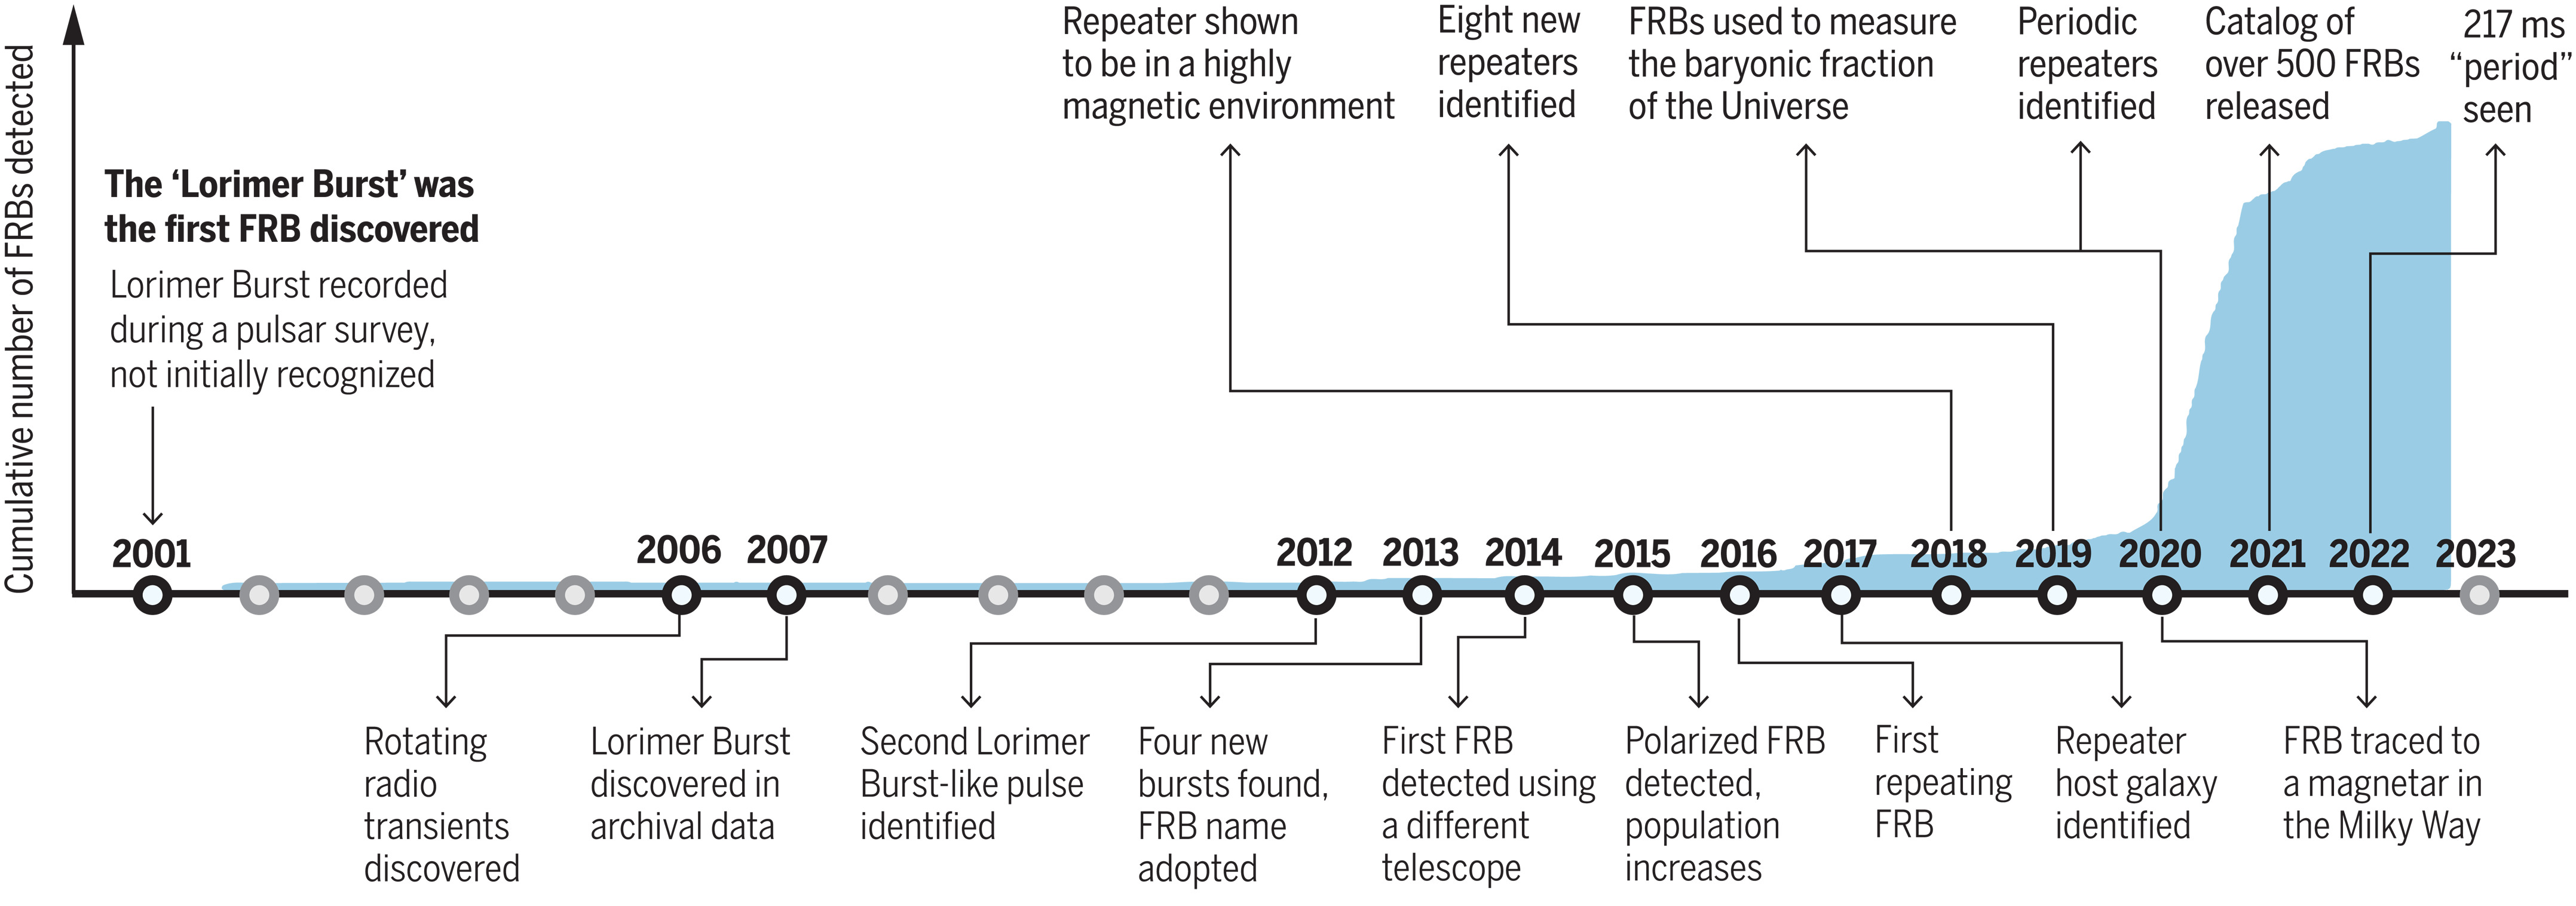
\includegraphics{././_assets/frb-research-review_C_Bailes2022.jpg}

\bookmarksetup{startatroot}

\hypertarget{properties-of-fast-radio-bursts}{%
\chapter{Properties of Fast Radio
Bursts}\label{properties-of-fast-radio-bursts}}

\hypertarget{observed-properties}{%
\section{Observed Properties}\label{observed-properties}}

\hypertarget{sec-prop-dm}{%
\subsection{Dispersion Measure}\label{sec-prop-dm}}

\hypertarget{intrinsic-width}{%
\subsection{Intrinsic Width}\label{intrinsic-width}}

\hypertarget{flux-density-and-fluence}{%
\subsection{Flux Density and Fluence}\label{flux-density-and-fluence}}

\hypertarget{derived-properties}{%
\section{Derived Properties}\label{derived-properties}}

\hypertarget{distance}{%
\subsection{Distance}\label{distance}}

\hypertarget{brightness-temperature}{%
\subsection{Brightness Temperature}\label{brightness-temperature}}

\hypertarget{luminosity}{%
\subsection{Luminosity}\label{luminosity}}

\bookmarksetup{startatroot}

\hypertarget{fast-radio-burst-population}{%
\chapter{Fast Radio Burst
Population}\label{fast-radio-burst-population}}

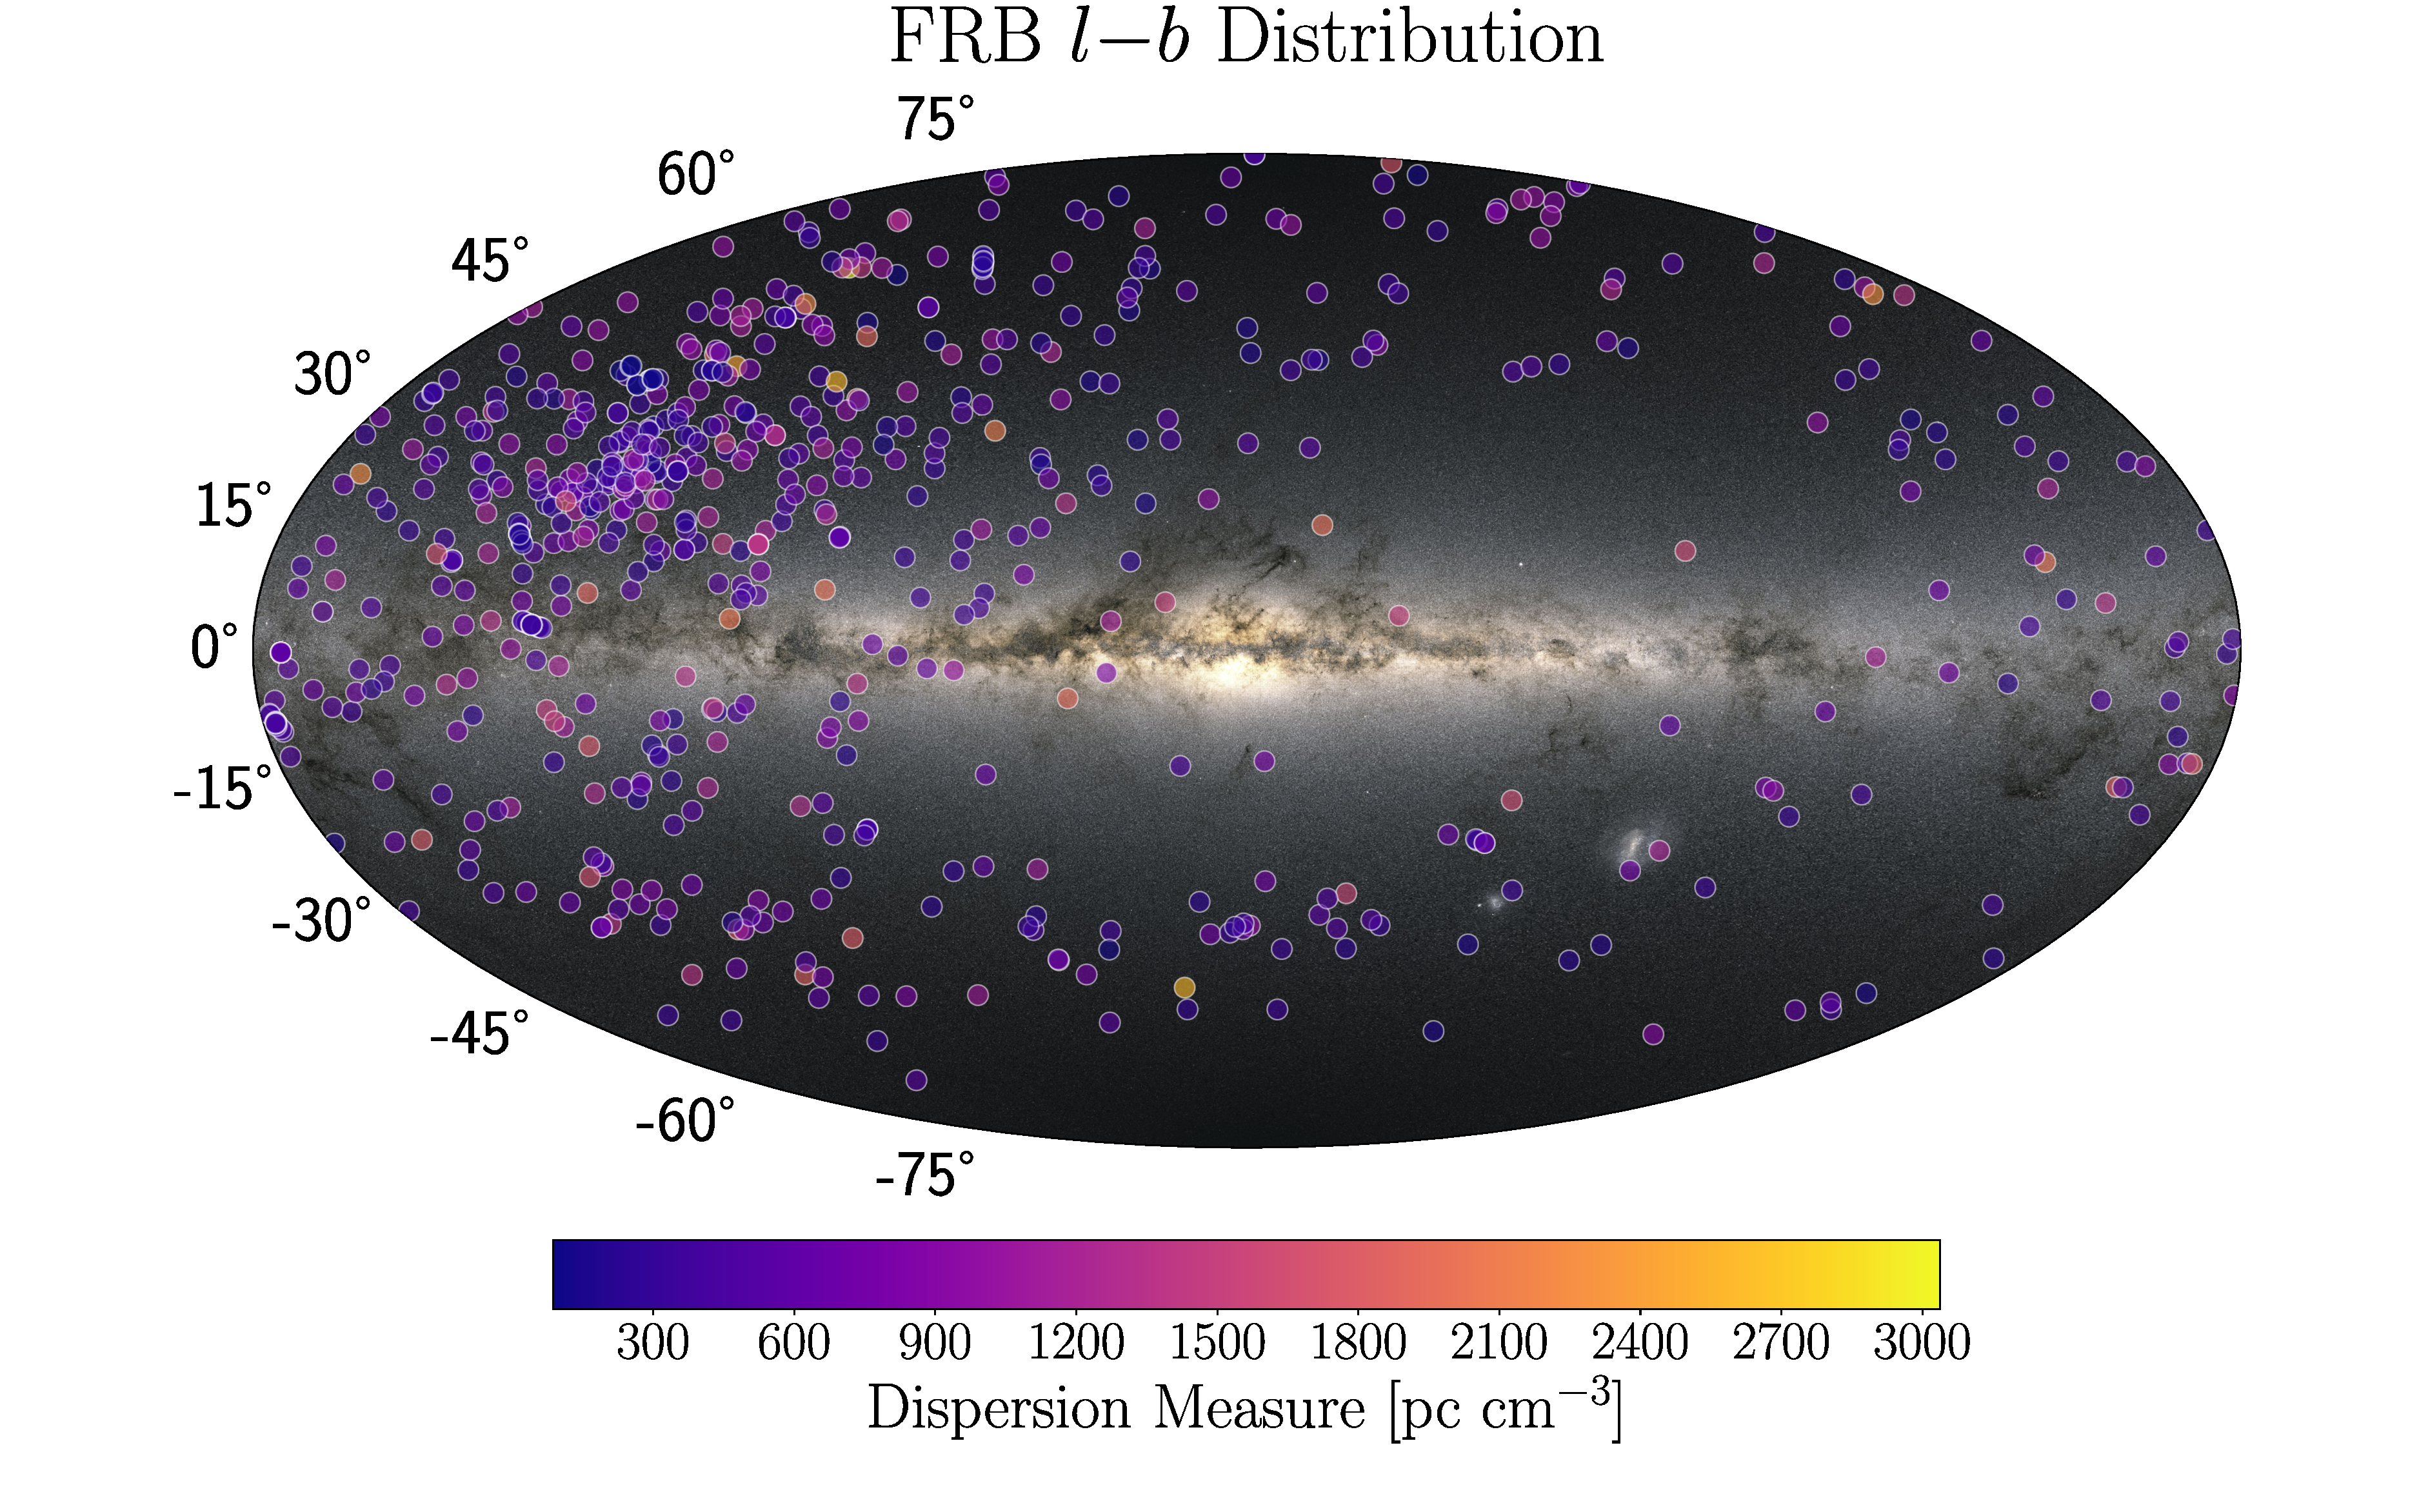
\includegraphics{././_assets/lat_long.svg}

\hypertarget{the-chimefrb-catalog}{%
\section{The CHIME/FRB Catalog}\label{the-chimefrb-catalog}}

The commisioning of the CHIME telescope with a FRB processing pipeline
(CHIME/FRB) marks the wealth of FRB data. CHIME/FRB has a wealth of
data. We can see that among the 818 FRBs detected, 632 (77.1\%) are
CHIME/FRB. Plus, among all of them, CHIME/FRBs data is more thorough
than others The CHIME/FRB Collaboration et al. (2021). The columns are
well documented etc and the whole dataset is available to
study\footnote{https://chime-frb-open-data.github.io/}.

\begin{figure}

{\centering \includegraphics{./population_files/figure-pdf/fig-count-by-telescope-output-1.pdf}

}

\caption[\label{fig-count-by-telescope}The number of FRBs detected by
individual telescope as reported in FRBSTATS
to illustrate the sheer dominance of FRBs detected the CHIME/FRB
telescope.]{\label{fig-count-by-telescope}The number of FRBs detected by
individual telescope as reported in FRBSTATS\footnotemark{}
to illustrate the sheer dominance of FRBs detected the CHIME/FRB
telescope.}

\end{figure}
\footnotetext{https://www.herta-experiment.org/frbstats/}

\hypertarget{repeating-and-non-repeating-frb}{%
\section{Repeating and Non-Repeating
FRB}\label{repeating-and-non-repeating-frb}}

\hypertarget{potentially-repeating-frb}{%
\section{Potentially Repeating FRB}\label{potentially-repeating-frb}}

The only obvious differentiation of FRB is whether it is seen to repeat
or not. Spanakis-Misirlis (2021) reports a total of 208 (25.3\%)
detections are associated with 24 repeater sources while 614 (74.7\%)
detections are non-repeating\footnote{https://www.herta-experiment.org/frbstats
  as of 14th Jan 2023}.

It is important to note that there is no guarantee that non-repeating
FRBs will not repeat. Authors such as Pleunis et al. (2021), Bo Han Chen
et al. (2021), Zhu-Ge, Luo, and Zhang (2022) and Luo, Zhu-Ge, and Zhang
(2022) tried to predict which non-repeating FRB has the potential to
repeat using differing strategies.

\hypertarget{using-machine-learning}{%
\subsection{Using Machine Learning}\label{using-machine-learning}}

Machine learning is a method to infer information from a set of data.
There are two main types of machine learning: supervised and
unsupervised learning (Vanderplas 2016). A supervised machine learning
algorithm involves using data labels to infer the relationships between
data features and labels. On the other hand, an unsupervised machine
learning algorithm infers the relationships between data features
without any reference to labels.

Bo Han Chen et al. (2021) uses unsupervised machine learning to uncover
hidden relationships between FRBs. Inferring relationships directly from
multi-dimensional features of FRBs is hard so they make use of a machine
learning technique called `dimensional reduction' where 13 features (10
observational + 3 model-dependent) are reduced to a 2-dimensional
projection space. The authors found that repeater FRBs tend to be very
close to each other in the projection space and concluded, with the help
of a clustering algortihm, that non-repeating FRBs which formed groups
with said repeaters are potentially repeating.

\begin{figure}

{\centering 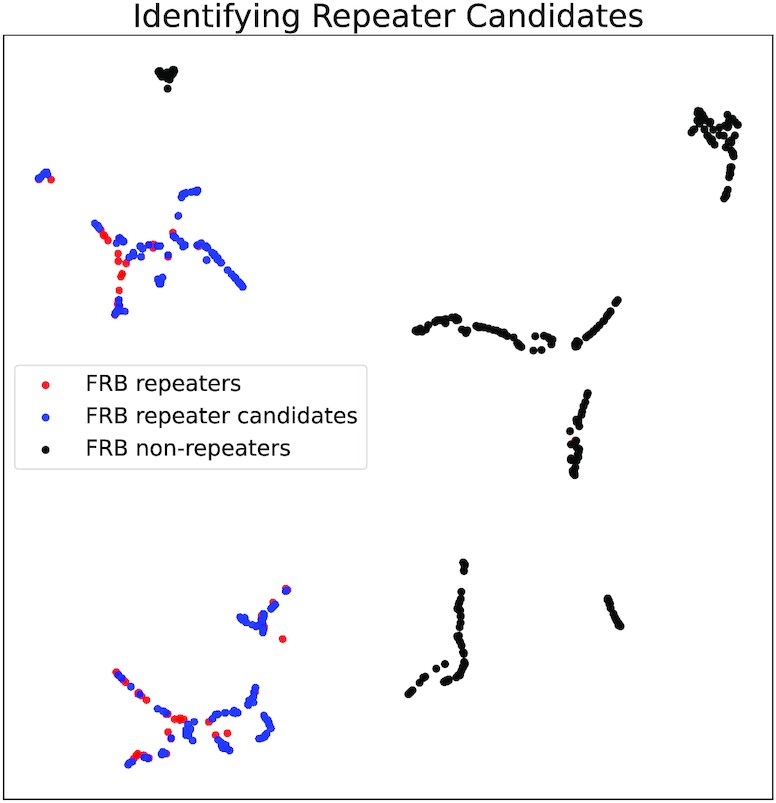
\includegraphics{././_assets/repeater-candidates_NC_Chen2022.jpg}

}

\caption{\label{fig-repeater-candidates-Chen2022}A 2D projection space
for 13 features of FRBs using the \emph{Uniform Manifold Approximation
and Projection} (UMAP) algorithm (McInnes, Healy, and Melville 2018).
Note that the x and y direction of a UMAP projection has no specific
meaning. However, the algorithm prioritizes preserving the local
structure of the data set therefore the formation of clumps means that
they are related to each other. The grouping is identified using
Hierarchical Density-Based Spatial Clustering of Applications with Noise
(HDBSCAN) (Campello, Moulavi, and Sander 2013). The 13 features are (i)
boxcar width, (ii) intrinsic width, (iii) peak flux, (iv) fluence, (v)
scattering time, (vi) spectral index, (vii) spectral running, (viii)
highest frequency, (ix) lowest frequency, (x) peak frequency, (xi)
redshift, (xii) radio energy, and (xiii) rest-frame intrinsic duration.
Parameters xi-xiii are model dependent.}

\end{figure}

Luo, Zhu-Ge, and Zhang (2022) and Zhu-Ge, Luo, and Zhang (2022) utilizes
both supervised and unsupervised learning with the methods split into
two papers. Their approach is not to choose any one particular algorithm
as a single model but uses multiple runs of multilple algorithms and
identify shared classifications. The supervised learning used by Luo,
Zhu-Ge, and Zhang (2022) includes decision tree method, random forest
method, support vector machine method, and the nearest centroid method;
where all of them are classification algorithms. The unsupervised
learning used by Zhu-Ge, Luo, and Zhang (2022) includes both dimensional
reduction algorithms and clustering algorithms similar to Bo Han Chen et
al. (2021) but different in the way that multiple algorithms of the same
task is used such as Pricipal Component Analaysis (PCA), T-distributed
Stochastic Neighbour Embedding (T-SNE), and UMAP for dimensional
reduction and k-means algorithm and HDBSCAN for the clustering
algorithm.

There is still no consensus on which model best fit the use case of
identifying potentially repeating FRBs. In spite of that, the fact that
algorithms can identify that repeaters are similar to each other than to
non-repeaters without knowledge of its repeating nature shows that there
is an underlying difference between repeaters and non-repeaters. It is
implied in all of the approaches Zhu-Ge, Luo, and Zhang (2022) that
potentially repeating FRBs have latent features of an identified
repeater.

\bookmarksetup{startatroot}

\hypertarget{references}{%
\chapter*{References}\label{references}}
\addcontentsline{toc}{chapter}{References}

\markboth{References}{References}

\hypertarget{refs}{}
\begin{CSLReferences}{1}{0}
\leavevmode\vadjust pre{\hypertarget{ref-bailes_discovery_FRB_2022}{}}%
Bailes, Matthew. 2022. {``The Discovery and Scientific Potential of Fast
Radio Bursts.''} \emph{Science} 378 (6620): eabj3043.
\url{https://doi.org/10.1126/science.abj3043}.

\leavevmode\vadjust pre{\hypertarget{ref-bohanchen_uncloaking_2021}{}}%
Bo Han Chen, Tetsuya Hashimoto, Tomotsugu Goto, Seong Jin Kim, Daryl Joe
D. Santos, Alvina Y. L. On, Ting-Yi Lu, and Tiger Y. -Y. Hsiao. 2021.
{``Uncloaking Hidden Repeating Fast Radio Bursts with Unsupervised
Machine Learning.''} \emph{Monthly Notices of the Royal Astronomical
Society} 509 (1): 1227--36.
\url{https://doi.org/10.1093/mnras/stab2994}.

\leavevmode\vadjust pre{\hypertarget{ref-campello_HDBSCAN_2013}{}}%
Campello, Ricardo J. G. B., Davoud Moulavi, and Joerg Sander. 2013.
{``Density-{Based Clustering Based} on {Hierarchical Density
Estimates}.''} In \emph{Advances in {Knowledge Discovery} and {Data
Mining}}, edited by Jian Pei, Vincent S. Tseng, Longbing Cao, Hiroshi
Motoda, and Guandong Xu, 160--72. Lecture {Notes} in {Computer Science}.
{Berlin, Heidelberg}: {Springer}.
\url{https://doi.org/10.1007/978-3-642-37456-2_14}.

\leavevmode\vadjust pre{\hypertarget{ref-hewish_rapidlyPulsating_1968}{}}%
Hewish, A., S. J. Bell, J. D. H. Pilkington, P. F. Scott, and R. A.
Collins. 1968. {``Observation of a {Rapidly Pulsating Radio Source}.''}
\emph{Nature} 217 (5130): 709--13.
\url{https://doi.org/10.1038/217709a0}.

\leavevmode\vadjust pre{\hypertarget{ref-lorimer_bright_2007}{}}%
Lorimer, D. R., M. Bailes, M. A. McLaughlin, D. J. Narkevic, and F.
Crawford. 2007. {``A Bright Millisecond Radio Burst of Extragalactic
Origin.''} \emph{Science} 318 (5851): 777--80.
\url{https://doi.org/10.1126/science.1147532}.

\leavevmode\vadjust pre{\hypertarget{ref-luo_machinelearningfrb_2022}{}}%
Luo, Jia-Wei, Jia-Ming Zhu-Ge, and Bing Zhang. 2022. {``Machine Learning
Classification of {CHIME} Fast Radio Bursts: {I}. {Supervised
Methods}.''} \emph{Monthly Notices of the Royal Astronomical Society},
November, stac3206. \url{https://doi.org/10.1093/mnras/stac3206}.

\leavevmode\vadjust pre{\hypertarget{ref-mcinnes_UMAP_2018}{}}%
McInnes, Leland, John Healy, and James Melville. 2018. {``{UMAP}:
{Uniform Manifold Approximation} and {Projection} for {Dimension
Reduction}.''} \emph{arXiv e-Prints}.

\leavevmode\vadjust pre{\hypertarget{ref-petroff_fast_2019}{}}%
Petroff, E., J. W. T. Hessels, and D. R. Lorimer. 2019. {``Fast Radio
Bursts.''} \emph{The Astronomy and Astrophysics Review} 27 (1): 4.
\url{https://doi.org/10.1007/s00159-019-0116-6}.

\leavevmode\vadjust pre{\hypertarget{ref-petroff_fast_2022}{}}%
---------. 2022. {``Fast Radio Bursts at the Dawn of the 2020s.''}
\emph{The Astronomy and Astrophysics Review} 30 (1): 49.
\url{https://doi.org/10.1007/s00159-022-00139-w}.

\leavevmode\vadjust pre{\hypertarget{ref-pleunis_fast_2021}{}}%
Pleunis, Ziggy, Deborah C. Good, Victoria M. Kaspi, Ryan Mckinven, Scott
M. Ransom, Paul Scholz, Kevin Bandura, et al. 2021. {``Fast {Radio Burst
Morphology} in the {First CHIME}/{FRB Catalog}.''} \emph{The
Astrophysical Journal} 923 (1): 1.
\url{https://doi.org/10.3847/1538-4357/ac33ac}.

\leavevmode\vadjust pre{\hypertarget{ref-spanakis-misirlis_frbstats_2021}{}}%
Spanakis-Misirlis, Apostolos. 2021. {``{FRBSTATS}: {A} Web-Based
Platform for Visualization of Fast Radio Burst Properties.''}
\emph{Astrophysics Source Code Library}, June, ascl:2106.028.
\url{https://ui.adsabs.harvard.edu/abs/2021ascl.soft06028S}.

\leavevmode\vadjust pre{\hypertarget{ref-stappers_pulsars_2011}{}}%
Stappers, B. W., J. W. T. Hessels, A. Alexov, K. Anderson, T. Coenen, T.
Hassall, A. Karastergiou, et al. 2011. {``Observing Pulsars and Fast
Transients with {LOFAR}.''} \emph{Astronomy \& Astrophysics} 530 (June):
A80. \url{https://doi.org/10.1051/0004-6361/201116681}.

\leavevmode\vadjust pre{\hypertarget{ref-the_chimefrbcollaboration_FirstCHIMEFRB_2021}{}}%
The CHIME/FRB Collaboration, Mandana Amiri, Bridget C. Andersen, Kevin
Bandura, Sabrina Berger, Mohit Bhardwaj, Michelle M. Boyce, et al. 2021.
{``The {First CHIME}/{FRB Fast Radio Burst Catalog}.''} \emph{The
Astrophysical Journal Supplement Series} 257 (2): 59.
\url{https://doi.org/10.3847/1538-4365/ac33ab}.

\leavevmode\vadjust pre{\hypertarget{ref-thornton_population_2013}{}}%
Thornton, D., B. Stappers, M. Bailes, B. Barsdell, S. Bates, N. D. R.
Bhat, M. Burgay, et al. 2013. {``A {Population} of {Fast} {Radio}
{Bursts} at {Cosmological} {Distances}.''} \emph{Science} 341 (6141):
53--56. \url{https://doi.org/10.1126/science.1236789}.

\leavevmode\vadjust pre{\hypertarget{ref-vanderplas_PythonDataScience_2016}{}}%
Vanderplas, Jacob T. 2016. \emph{Python Data Science Handbook: Essential
Tools for Working with Data}. First edition. {Sebastopol, CA}: {O'Reilly
Media, Inc}.

\leavevmode\vadjust pre{\hypertarget{ref-zhuge_machinelearningfrb_2022}{}}%
Zhu-Ge, Jia-Ming, Jia-Wei Luo, and Bing Zhang. 2022. {``Machine
{Learning Classification} of {Fast Radio Bursts}: {II}. {Unsupervised
Methods}.''} {arXiv}. \url{https://doi.org/10.48550/arXiv.2210.02471}.

\end{CSLReferences}



\end{document}
